\bgroup
\def\arraystretch{1.5}
\begin{figure*}[tp]
	\begin{center}
		\begin{tabular}{c|ccccccc}
			\textbf{Original} & \multicolumn{7}{c}{\textbf{Rotated}} \\
			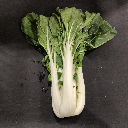
\includegraphics[scale=0.4]{./img/bokchoi_0.png} &
			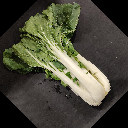
\includegraphics[scale=0.4]{./img/bokchoi_1.png} &
			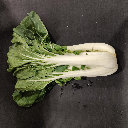
\includegraphics[scale=0.4]{./img/bokchoi_2.png} &
			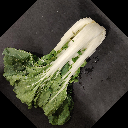
\includegraphics[scale=0.4]{./img/bokchoi_3.png} &
			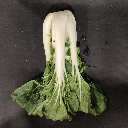
\includegraphics[scale=0.4]{./img/bokchoi_4.png} &
			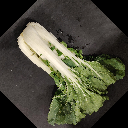
\includegraphics[scale=0.4]{./img/bokchoi_5.png} &
			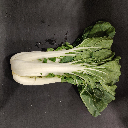
\includegraphics[scale=0.4]{./img/bokchoi_6.png} &
			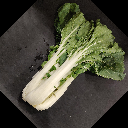
\includegraphics[scale=0.4]{./img/bokchoi_7.png} \\
			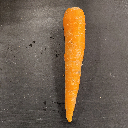
\includegraphics[scale=0.4]{./img/carrot_0.png} &
			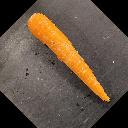
\includegraphics[scale=0.4]{./img/carrot_1.png} &
			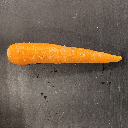
\includegraphics[scale=0.4]{./img/carrot_2.png} &
			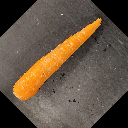
\includegraphics[scale=0.4]{./img/carrot_3.png} &
			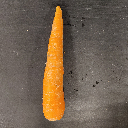
\includegraphics[scale=0.4]{./img/carrot_4.png} &
			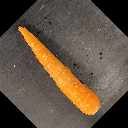
\includegraphics[scale=0.4]{./img/carrot_5.png} &
			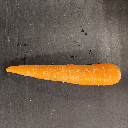
\includegraphics[scale=0.4]{./img/carrot_6.png} &
			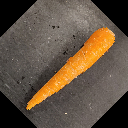
\includegraphics[scale=0.4]{./img/carrot_7.png} \\
		\end{tabular}
		\label{tab:veg_types}
	\end{center}
	\caption{Two sample images with their rotated counterparts.}
	\label{fig:veg_rotations}
\end{figure*}
\egroup

For the validation of the proposed feature augmented classifier, we create a dataset of 24 fruits and vegetables (see Table \ref{tab:veg_types}). We capture 10 RGB images of $128 \times 128$ pixels for each type of fruit or vegetable. The RGB format is used as it is a real colour format for an image \cite{b3_1}. Each of these images are rotated 7 times to create new images, resulting in a total of 1920 RGB images for training.

As Fig. \ref{fig:veg_rotations} shows, the 7 rotations are applied at increasing increments of 45\degree{} starting from the original image. We do this to account for non-symmetric fruits and vegetables that are not axis aligned.

\bgroup
\def\arraystretch{1.5}
\begin{table}[htbp]
	\caption{Types of Fruits and Vegetables Used for Creating the Dataset}
	\begin{center}
		\begin{tabular}{| >{\centering\arraybackslash}m{2cm} | >{\centering\arraybackslash}m{2cm} | >{\centering\arraybackslash}m{2cm} |}
			\hline
			Cabbage & Bok Choi & Pear \\
			\hline
			Tomato & Brussel Sprout & Apple \\
			\hline
			Orange Pepper & White Turnip & Potato \\
			\hline
			Red Pepper & Okra & Lemon \\
			\hline
			Jalapeño & Eggplant & Plantain \\
			\hline
			Green Pepper & Squash Zucchini & Kiwi \\
			\hline
			Beet & Carrot & Onion \\
			\hline
			Daikon Lo Bok & Orange & Mango \\
			\hline
		\end{tabular}
		\label{tab:veg_types}
	\end{center}
\end{table}
\egroup